%! Licence = CC BY-NC-SA 4.0

%! Author = gianfluetsch, mariuszindel
%! Date = 30. Dez 2021
%! Project = cydef_summary

\section{Begriffe}\label{sec:Begriffe}

\subsection{SIEM: Security Information and Event Management}\label{subsec:siem}
Sicherheitsinformationen und Ereignisverwaltung aus verschiedenen Quellen (Netzwerk, Servern, Anwendungen, \ldots) in Echtzeit aggregieren, identifizieren, kategorisieren und analysieren.\\
Sicherheitsprobleme sollten automatisch erkannt und eine Warnung versenden werden.
\subsubsection{Vorteile}
\begin{itemize}
    \item Ermöglicht die Mustersuche in Protokolldaten nach Indikatoren für einen Cyberangriff (IOC)
    \item Ermöglicht die Korrelation von Ereignisinformationen und identifiziert abnormale Aktivitäten
    \item Alarme nach definierten Alarmregeln
\end{itemize}

\subsubsection{Nachteile}
\begin{itemize}
    \item Kann sehr komplex sein
    \item Implementierung kann lange dauern (hoher Aufwand)
    \item oft kostspielig, da nicht direkt ,,out of the box``
\end{itemize}

\subsubsection{Anwendungen / Hersteller}
\begin{itemize}
    \item Wazuh
    \item Splunk
    \item Exabeam
\end{itemize}


\subsection{SOAR: Security Orchestration, Automation \& Response Solutions}\label{subsec:soar}
SOAR sammelt ebenfalls Daten aus verschiedenen Quellen, ähnlich wie ein SIEM.
SOAR unterstützt ein Incident Responder bei der Bewältigung des Vorfalls. SOAR ermöglicht ein automatisiertes Eingreifen, wenn ein Sicherheitsvorfall eintritt. Ein SOAR-System unterstützt den Incident Responder auch bei der Einführung von Sicherheits Gegenmaßnahmen (Active Directory).\\

\subsubsection{Vorteile}
\begin{itemize}
    \item Alert Investigation
    \item Orchestration
    \item Automatisierter Workflow: schnellere Reaktion bei Vorfällen und deren Behebung
    \item höhere Produktivität
    \item weniger langwierige und sich wiederholende Tätigkeiten für die Fachkräfte
\end{itemize}

\subsubsection{Nachteile}
\begin{itemize}
    \item Hat auf jedem Client hohe Rechte $\rightarrow$ kann auch angegriffen werden.
    \item Kann die ,,Sicherheitsreife`` im Unternehmen nicht beurteilen oder Änderungen berücksichtigen
    \item Wurde eine Sicherheitskultur nicht etabliert, helfen auch die Tools nicht
    \item begrenzte oder unklare Erfolgsmetriken
    \item Umschichtung von Personalressourcen auf Technologieressourcen
\end{itemize}

\subsubsection{Anwendungen / Hersteller}
\begin{itemize}
    \item Velociraptor
\end{itemize}


\vfill
$ $
\columnbreak


\subsection{EDR: Endpoint Protection and Response}\label{subsec:edr}
Endpoint Detection and Response (EDR), auch bekannt als Endpoint Threat Detection and Response (ETDR), ist eine integrierte Endpunkt-Sicherheitslösung, die eine kontinuierliche Überwachung und Erfassung von Endpunktdaten in Echtzeit mit regelbasierten automatischen Reaktions- und Analysefunktionen
EDR wird direkt auf dem Client installiert, SOAR auf einem Server im Netzwerk. Kann mit einem Antivirus Programm verglichen werden.

\subsubsection{Vorteile}
\begin{itemize}
    \item Sehr nahe beim Client, daher so schnell
\end{itemize}

\subsubsection{Nachteile}
\begin{itemize}
    \item Beweisvernichtung
    \item Benötigt Ressourcen auf dem Client
    \item Benötigt hoche Rechte auf Client
\end{itemize}

\subsubsection{Anwendungen / Hersteller}
\begin{itemize}
    \item Microsoft
    \item CrowdStrike
    \item Trend Micro
\end{itemize}


\subsection{CERT: Computer Emergency Response Team}
% TODO: More Information?
% https://www.techtarget.com/searchsecurity/tip/CERT-vs-CSIRT-vs-SOC-Whats-the-difference
Das CERT ist eine Gruppe von IT-Sicherheitsfachleuten, die sowohl präventive als auch reaktive Maßnahmen bei sicherheitsrelevanten Vorfällen in Computer-Systemen empfiehlt.
Sie wirken an der Lösung von konkreten Sicherheitsvorfällen mit, liefern Lösungsansätze oder warnen vor Sicherheitslücken.
Eine andere Bezeichnung für Computer Emergency Response Team ist CSIRT (Computer Security Incident Response Team).

\begin{itemize}
    \item Trademark
    \item Unpräzise
\end{itemize}

\subsection{CSIRT: Computer Emergency Security Incident Response Team}\label{subsec:csirt}
Ein CSIRT ist ein Team von IT-Sicherheitsexperten, dessen Hauptaufgabe darin besteht, auf Computersicherheitsvorfälle zu reagieren. Es bietet die notwendigen Dienstleistungen an, um diese zu bearbeiten und die Betroffenen bei der Wiederherstellung nach Verstössen zu unterstützen.

\begin{itemize}
    \item Präziser
    \item Free to use
    \item 19 Teams in CH
\end{itemize}
 Wird oft als synonym verwendet zu CERT

\subsection{SOC}\label{subsec:soc}
Der Aufgabenbereich eines SOC kann sowohl Incident Response (ganz oder teilweise) als auch andere Aufgaben umfassen, z.B.:

\begin{itemize}
    \item Überwachung von Abläufen und Kontrollen (z.B. Intrusion Detection / Intrusion Prevention System, etc.)
    \item die Auswertung von Betriebs- und Sicherheitstelemetrie und Informationserfassung beaufsichtigen
    \item Verwaltung von Aufgaben wie Identitätsmanagement und Autorisierung, Wartung von Firewall- und Filterregeln (sowohl Überprüfung als auch Änderungsverwaltung)
    \item forensische und investigative Unterstützung oder andere Aspekte der operativen Sicherheit.
\end{itemize}

\begin{center}
    \vspace{-8pt}
    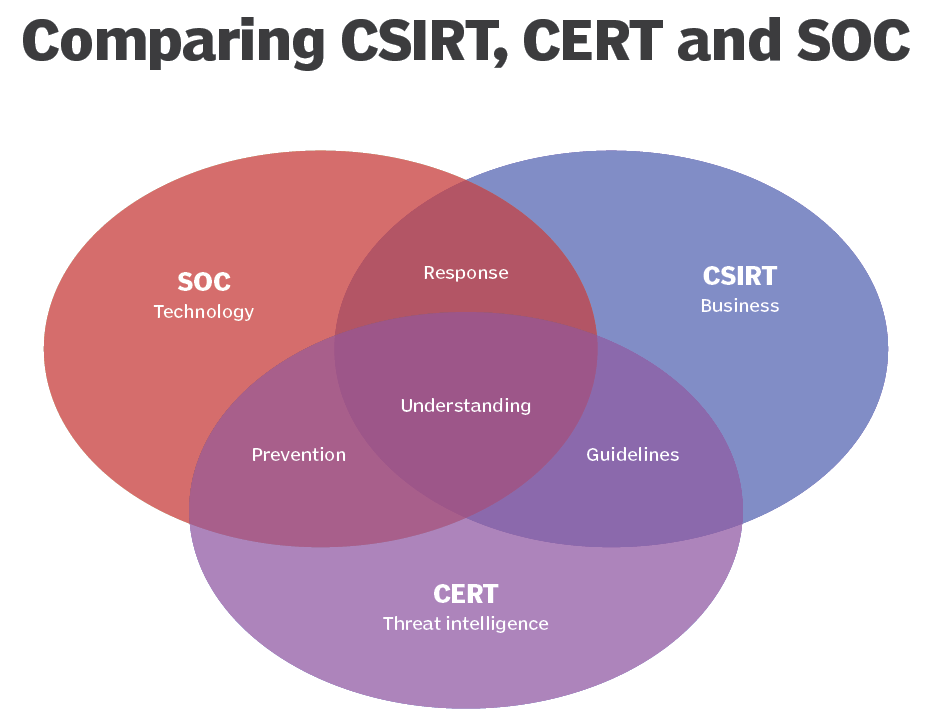
\includegraphics[width=0.8\linewidth]{./img/02-begriffe/soc_cert_csirt}
    \vspace{-8pt}
\end{center}

\subsection{IOC: Indices of Compromize}
Indicators of Compromise (IOCs) definieren die Merkmale eines Vorfalls auf strukturierte Weise. Sie haben das Ziel, Artefakte im Zusammenhang mit Vorfällen zu beschreiben und zu finden.
\textbf{Format:}
\begin{itemize}
    \item Host-basierte IOC-Formate (noch kein akzeptierter Standard)
    \begin{itemize}
        \item YARA
        \item STIX, TAXII
        \item Mandiant's OpenIOX
    \end{itemize}
    \item Netzbasierte IOC-Formate
    \begin{itemize}
        \item Snort rules
    \end{itemize}
\end{itemize}

\subsection{Incident Response}
% TODO: Include content here or somwhere else?
% NIST
% SANS

\subsection{NIST vs. SANS}
\begin{center}
    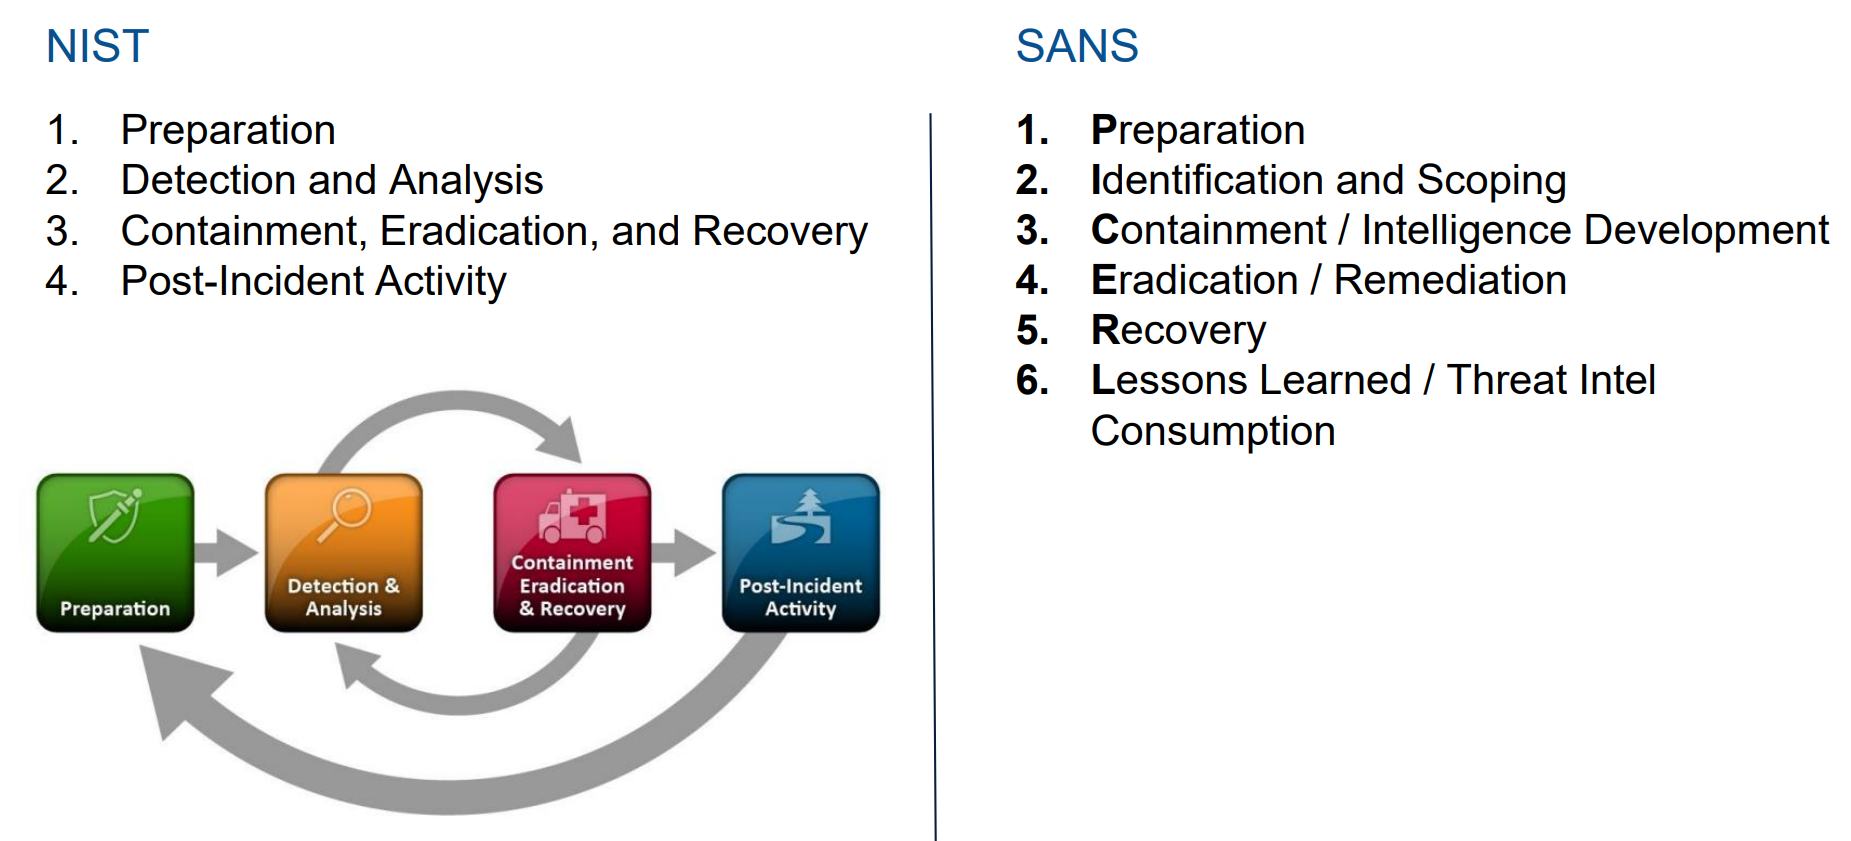
\includegraphics[width=1.0\linewidth]{./img/02-begriffe/nist_sans}
\end{center}



\subsubsection{Sigma}
Sigma ist ein generisches und offenes Signaturformat, mit dem Sie relevante Protokollereignisse auf einfache Weise beschreiben können. Das Regelformat ist sehr flexibel, leicht zu schreiben und auf jede Art von Protokolldateien anwendbar. Das Hauptziel dieses Projekts ist es, eine strukturierte Form bereitzustellen, in der Forscher oder Analysten ihre einmal entwickelten Erkennungsmethoden beschreiben und mit anderen teilen können.\\
\textit{Sigma} ist für Logs das, was Snort für den Netzwerkverkehr und YARA für Dateien ist.\\
\textbf{Use-Cases}
\begin{itemize}
    \item Describe your detection method in Sigma to make it shareable
    \item YAML based
    \item Write your SIEM searches in Sigma to avoid a vendor lock-in
    \item Share the signature in the appendix of your analysis along with IOCs and YARA rules
    \item Share the signature in threat intel communities - e.g. via MISP
    \item Provide Sigma signatures for malicious behaviour in your own application
\end{itemize}



%TODO Include Lab solution